\documentclass[letterpaper, 12pt]{math}

\usepackage{listings}
\lstset{basicstyle=\ttfamily\footnotesize,breaklines=true}
\usepackage{pgfplots}
\pgfplotsset{compat=1.8}

\title{Analysis of Algorithms}
\author{Alvin Lin (axl1439) and William Leuschner (wel2138)}
\date{August 2017 - December 2017}

\begin{document}

\maketitle

\section*{Problem 1}

\subsubsection*{Algorithm Description}
For this problem, we used a dynamic programming solution to find the maximum
number of classes that can fit into a schedule, allotting for travel time.
During each step, it computes the maximum number of classes that can be taken
from among the current subset of classes. It finds the largest previous
solution, then adds one and sets that value as the current solution, but only
if that largest solution fit before the current interval. If it was unable to
find a previous solution that fit before the current interval, then the current
solution is simply one, consisting only of the the current interval.

\subsubsection*{Argument of Correctness}
Heart of the solution:
\begin{align*}
  \texttt{S[i]} =& \text{ the maximum number of non-overlapping classes} \\
  & \text{(including travel time) from the set } a_{1}\dots a_{j}
\end{align*}
To calculate \texttt{S[i]}:
\[ \text{Let } \texttt{index} = \texttt{max(S[:i-1])} \text{ such that }
  a_{\texttt{index}}.end + \text{travel time} \le a_{\texttt{i}}.start \]
\[ \texttt{S[i]} = \texttt{S[index]} + 1 \text{ if such an index exists,
  otherwise } 1 \]
\[ \texttt{S[1] = 1} \]

\subsubsection*{Running Time Estimate}
This algorithm needs to iterate through each interval, and during each
iteration needs to find the maximum previous solution. This makes it
\( O(n^2) \).

\subsubsection*{Pseudocode}
\begin{lstlisting}
def getEndTimeWithTravel(startClass, endClass, travelTimes):
    return startClass.endTime +
        travelTimes[startClass.index][endClass.index]

def findGreatestNumberOfIntervals(intervals, travelTimes):
    intervals = heapSort(intervals, keeping track of original index)
    let solution = [] of size intervals.length
    solution[0] = 1
    for i = 1 to intervals.length:
        let current = intervals[i]
        solution[i] = 1
        for j = 0 to i:
            tmp = intervals[j]
            if solution[j] >= solution[i] and
                getEndTimeWithTravel(tmp, current, travelTimes):
                solution[i] = solution[j] + 1
    return max(solution)
\end{lstlisting}

\section*{Problem 2}
For this problem, we implemented both the recursive solution and the dynamic
programming solution.
\begin{center}
  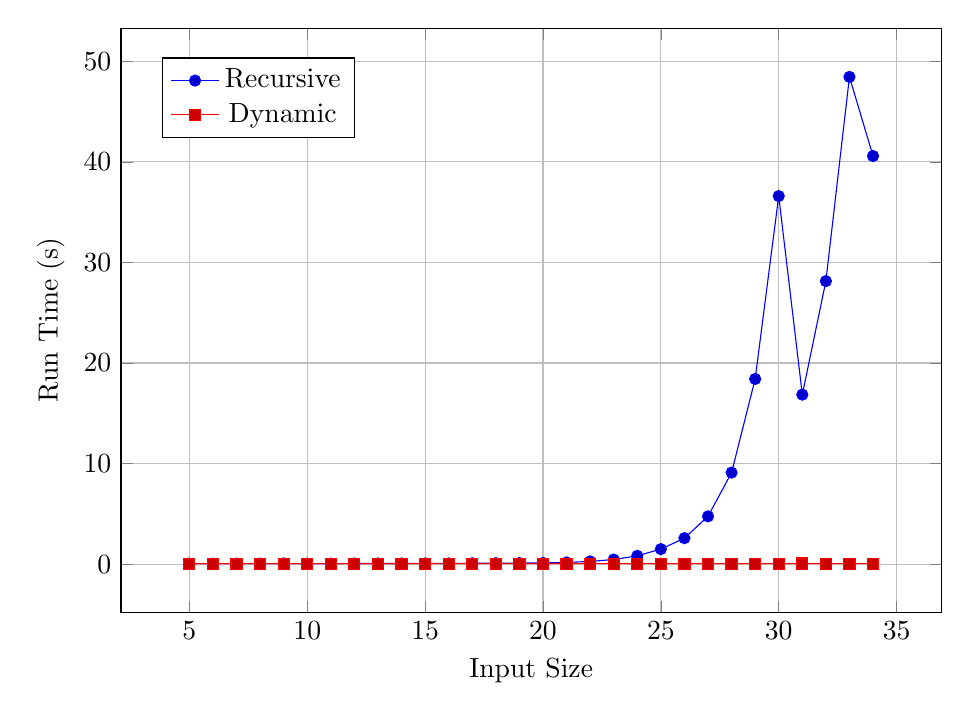
\begin{tikzpicture}
    \begin{axis}[height=9cm, width=12cm, grid=major,
        legend style={at={(0.05,0.95)},anchor=north west},
        xlabel=Input Size, ylabel=Run Time (s)
      ]
      \addplot coordinates {
        (5,0.059) (6,0.053) (7,0.056) (8,0.056) (9,0.064) (10,0.055) (11,0.055)
        (12,0.065) (13,0.068) (14,0.071) (15,0.075) (16,0.075) (17,0.087)
        (18,0.100) (19,0.110) (20,0.128) (21,0.173) (22,0.274) (23,0.460)
        (24,0.830) (25,1.497) (26,2.587) (27,4.753) (28,9.104) (29,18.413)
        (30,36.596) (31,16.855) (32,28.140) (33,48.443) (34,40.577)
      };
      \addlegendentry{Recursive}
      \addplot coordinates {
        (5,0.049) (6,0.051) (7,0.054) (8,0.050) (9,0.056) (10,0.051) (11,0.052)
        (12,0.051) (13,0.050) (14,0.052) (15,0.050) (16,0.051) (17,0.055)
        (18,0.050) (19,0.054) (20,0.052) (21,0.050) (22,0.053) (23,0.050)
        (24,0.057) (25,0.050) (26,0.050) (27,0.052) (28,0.053) (29,0.049)
        (30,0.051) (31,0.060) (32,0.052) (33,0.057) (34,0.058)
      };
      \addlegendentry{Dynamic}
    \end{axis}
  \end{tikzpicture}
\end{center}
The recursive solution is significantly slower than the dynamic programming
solution.

\section*{Problem 3}

\subsubsection*{Part 1 Psuedocode}
\begin{lstlisting}
def longestIncreasingSubsequence(sequence, start):
    if start == sequence.length - 1:
        return sequence[-1:]
    minVal = sequence[start]
    minIndex = start
    for i = start to sequence.length:
        if sequence[i] < minVal:
            minVal = sequence[i]
            minIndex = i
    return [minVal] + [findNextItem(sequence, minIndex + 1)]
\end{lstlisting}

\subsubsection*{Part 1 Running Time Estimate}
\[ O(n^2) \]

\subsubsection*{Part 1 Counterexample}
Sequence: [5, 6, 7, 8, 9, 0, 1, 2, 3] \\
Greedy Algorithm Output: [0, 1, 2, 3] \\
Optimal Solution: [5, 6, 7, 8, 9]

\subsubsection*{Part 2 Pseudocode}
\begin{lstlisting}
def longestIncreasingSubsequence(sequence, start):
    let num_loops = 0
    let subsequences = []
    for l = 0 to sequence.length:
        num_loops += 1
        let i = l
        subsequence = []
        subsequence.append(sequence[l])
        while i < sequence.length:
            num_loops += 1
            if sequence[i] < sequence[j]:
                subsequence.append(sequence[j])
                i = j
                break
            if j == sequence.length - 1:
                i = sequence.length
                break
        subsequences.append(subsequence)
    sort = sorted(subsequences by length of subsequences from max to min)
    return sort[0]
\end{lstlisting}

\subsubsection*{Part 2 Running Time Estimate}
\[ O(n^2) \]

\subsubsection*{Part 2 Counterexample}
Sequence: [1, 8, 3, 6, 5, 4, 7, 2, 9] \\
Greedy Algorithm Output: [3, 6, 7, 9] \\
Optimal Solution: [1, 3, 5, 7, 9]

\section*{Problem 4}

\subsubsection*{Algorithm Description}
For this problem, we implemented a dynamic programming solution that computed
the solution by building it one interval at a time. It computes the maximum
number of possible non-overlapping interval subsets at each step and subtracts
the number of overlaps the new interval has with the current solution.

\subsubsection*{Argument of Correctness}
Given a single interval \( i_1 \), the number of non-overlapping interval
subsets \texttt{S[1]} is two, consisting of the sets \( \emptyset,\{i_1\} \).
If we add a second interval \( i_2 \) that does not overlap with \( i_1 \),
then the number of\ solutions \texttt{S[2]} is 4, or \( 2\texttt{S[1]} \),
consisting of the interval subsets \( \emptyset,\{i_1\},\{i_2\},\{i_1,i_2\} \).
If interval \( i_2 \) does overlap with \( i_1 \), then we subtract the number
of intervals it overlaps with, making the solution \( 2\texttt{S[1]}-1 \), which
consists of the intervals \( \emptyset,\{i_1\},\{i_2\} \). The solution
\texttt{S[n]} with \( n \) intervals \( i_1,i_2,\dots,i_n \) can be
generalized inductively as:
\[ \texttt{S[n]} =
  2\texttt{S[n-1]}-i_n\text{'s overlaps with previous solution} \]
where:
\[ \texttt{S[0]} = 1 \]

\subsubsection*{Running Time Estimate}
This algorithm runs a single pass through all the intervals, and on each
interval it must calculate the number of overlaps with all the intervals in
the current solution. This makes it \( O(n^2) \).

\subsubsection*{Psuedocode}
\begin{lstlisting}
def countIntervals(intervals):
  let solution = 1
  for i = 1 to intervals.length:
    solution *= 2
    for j = 1 to i:
      if interval[i] overlaps interval[j]:
        solution -= 1
  return solution
\end{lstlisting}

\end{document}
